\documentclass{rapportECL}



% ------------- Packages spéciaux, nécessaires pour ce rapport, à insérer ici ------------- 
%\usepackage{lipsum}
\usepackage{booktabs} % table

\usepackage{minted}
%https://www.overleaf.com/learn/latex/Code_Highlighting_with_minted

%https://www.overleaf.com/latex/examples/source-code-highlighting-with-minted-in-latex/qphhfvnsddbs


 
%\usepackage{listingsutf8} %Display code in LaTeX, using the lstlisting environment
% https://tex.stackexchange.com/questions/312429/an-error-appears-saying-that-utf8-and-listing-are-not-compatible?rq=1

% to customize the three basic list environments (enumerate, itemize and description) and to design your own lists, with a <key>=<value> syntax.
% https://tex.stackexchange.com/questions/48036/how-to-represent-cross-and-tick-in-itemize-bullets
\usepackage{enumitem} %\begin{itemize}[label=$\star$]

%\setlist[itemize,1]{label=$\bullet$}
\setlist[itemize,2]{label=$\circ$}
\setlist[itemize,3]{label=$\diamond$}



\title{Rapport BE Colonie des Fourmis} %Titre du fichier

\begin{document}

%----------- Informations du rapport ---------

\titre{Rapport BE Colonie des Fourmis - } %Titre du fichier .pdf
\UE{UE INF} %Nom de la UE
\sujet{S8 Algorithmes collaboratifs et applications} %Nom du sujet

\enseignant{Alexander \textsc{SAIDI}} %Nom de l'enseignant

\eleves{Achraf \textsc{Bella} \\
		Bruno \textsc{Moreira Nabinger} } %Nom des élèves

%----------- Initialisation -------------------
        
\fairemarges %Afficher les marges
\fairepagedegarde %Créer la page de garde
\tabledematieres %Créer la table de matières

%------------ Corps du rapport ----------------


\section{Introduction} 

 L'objectif de ce Bureau d'Études (BE) est de réaliser l’implémentation d’un système multi-agents de recherche du chemin le plus court (PCC) suivant le principe de la stigmergie et utilisant les algorithmes génétiques. Basée sur la modélisation initiale de la colonie de fourmis présente en cours, une application a été développe pour permettre de résoudre plusieurs problèmes de recherche du PCC. On souhaite aussi étudier les comportement des algorithmes génétiques dans ce cas d'implémentation. L'un des objectifs spécifiques est donc de d'avoir un logicielle dont les paramétrés de simulation sont facilement réglables. Ainsi, une interface graphique a été développé.

% \section{Cahier des charges}

% Le cahier des charges est le suivant :

% \begin{itemize}
%     \item gestion du score et de l'historique des parties pour les joueurs ;
%     \item le clavier doit désactiver les touches déjà utilisées ;
%     \item les éléments du pendu doivent apparaître au fur et à mesure des échecs du joueur ;
%     \item un message de félicitations doit être affiché en cas de victoire et la réponse en cas de défaite .
% \end{itemize}

\section{Principe des Solutions}

%slide 19



\subsection{Les agents en IA}

\begin{itemize}[label=$\bullet$]
    \item Soit une route qui lie deux villes v1 et v2 :
    \begin{itemize}
        \item On fera "avancer" les fourmis \textbf{pas à pas}.
        \begin{itemize}
            \item un pas d’itération fera avancer \textit{d’un pas} chaque fourmi
        \end{itemize}
        \item Suite à ce "pas", on modifie l’état de l’agent (fourmi).
    \end{itemize}
\end{itemize}

\subsection{Le comportement d’un agent}

Le tableau \ref{tab:Description_des_action_dun_agent_en_fonction_de_chaque_etat} décrit les actions d’un agent en fonction de chaque Etat.

%https://www.tablesgenerator.com/

% Please add the following required packages to your document preamble:
% \usepackage{booktabs}
\begin{table}[H]
\centering
\begin{tabular}{@{}ll@{}}
\toprule
Lieu                                  & Actions                                           \\ \midrule
Dans une ville (noeud)                & Choisir l’arête suivante, déposer de la phéromone \\
Sur une route (arête)                 & Avancer un pas de plus                            \\
Au nid, transportant de la nourriture & Laissez les aliments                              \\
A la source de nourriture             & Prendre de l’aliment et retourner au nid          \\ \bottomrule
\end{tabular}
\caption{Description des actions d’un agent en fonction de chaque état}
\label{tab:Description_des_action_dun_agent_en_fonction_de_chaque_etat}
\end{table}

\begin{itemize}[label=$\bullet$]
    \item Un agent sur un itinéraire avance d’un pas (une étape) à chaque tour jusqu’à ce qu’il arrive dans une ville.
    \item Une fois dans la ville, il choisit un itinéraire en fonction de l’intensité de la
phéromone sur les chemins disponibles.
    \item Si l’agent trouve la source de nourriture ; il prend la nourriture puis démarre le
voyage de retour en suivant sa propre piste de phéromone ;
    \item De retour dans le nid, l’agent laisse la nourriture puis recommence le processus
à nouveau.
\end{itemize}

Notons qu’à chaque départ, les agents suivent les pistes ayant un maximum de phéromone. Mais au départ du nid, ils n’ont plus la mémoire de leur "propre" piste.

Notez que toutes ces actions nécessitent des informations locales et une mémoire à court terme permettant à l’agent de reconnaître son propre chemin vers le nid.

\section{Explication de l'interface}

Explication de l’utilisation de l’interface : 

Dans l’interface nous avons implanter 6 boutons chacun à son fonctionnement 
Le premier bouton c’est pour créer un environnement
Le deuxième bouton c’est pour importer un environnement déjà exister dans l’ordinateur
Le troisième buton c’est une démonstration pour montrer à l’utilisateur que le programme ça marche bien.
Le buton description pour avoir une idée sur le fonctionnement de l’application 
Et puis deux boutons crédits et quitter.
 
 \begin{figure}[H]
    \centering
    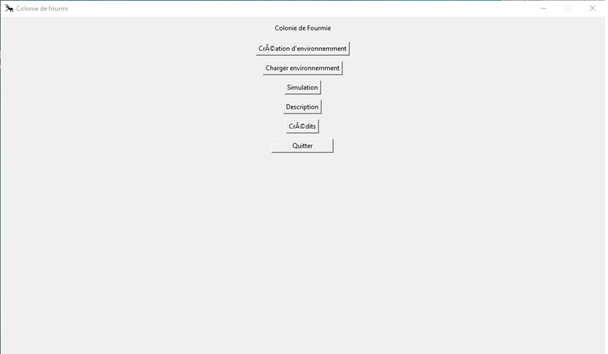
\includegraphics[width=0.8\linewidth]{1.png}
    \caption{ l'interface de l'utilisateur }
    \label{Dim}
\end{figure}\\
 
Pour générer un graphe il suffit de click sur l’interface et définir les villes comme montre la figure suivante 

 \begin{figure}[H]
    \centering
    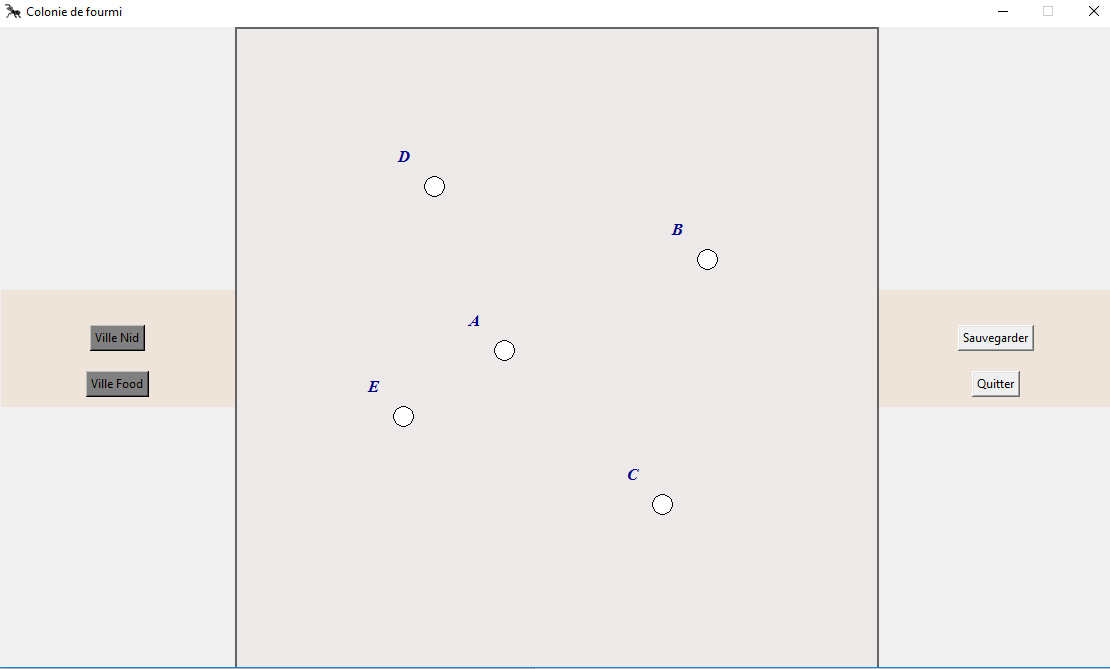
\includegraphics[width=0.8\linewidth]{2.png}
    \caption{ Ville dans l'interface }
    \label{Dim}
\end{figure}\\

Puis il faut définir pour les relations entre les villes pour cela il suffit de cliquer sur une ville pour être sure la couleur de la ville tourne en orange puis cliquant sur une autre ville pour définir la relation comme montre la figure.

 \begin{figure}[H]
    \centering
    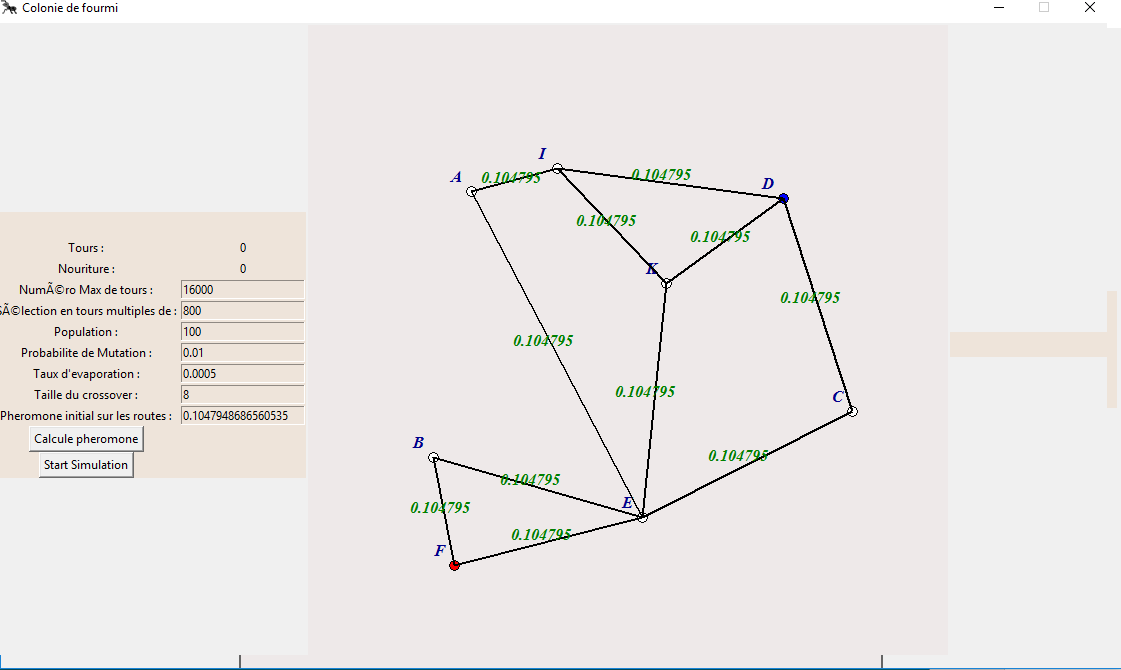
\includegraphics[width=0.8\linewidth]{3.png}
    \caption{ exemple d'exusion de programme }
    \label{Dim}
\end{figure}\\

Dans l’interface nous avons le nombre de tours qui correspond à un pas dans fait par une fourni, en ce qui concerne la nourriture en le comptabilise à chaque fois une fourni trouver sans chemin de retour.
Aussi le bouton population qui définir le nombre des agents pour notre cas c’est le nombre des fourni 
Le bouton de probabilité de mutation fonction comme suivant en générer un nombre alectorie si c’est plus grand que la probabilité donnée en fait une mutation à la fourni.
Le taux d’évaporation représente le processus d’évaporation chez les fournis, qui est une fonction décroissante sous forme de X   expo(-X)    
Taille de Croissover pour définir le nombre des agents pour faire le croissement.

\section{Algorithme Génétique}

Pour exécuter le programme il faut être conscient de quelque anomalie.
Dans un graphe qui contient un sous graphe fermé et qui ne contient pas ni de ville de nid ou de ville 
de source il y a des fournis qui perdre leur chemin c’est-à-dire il font des tours infinis jusqu’à
L’algorithme élimine les fournis qui ne revient pas au nid.\\

Il faut assurer que le graphe choisi ne doit pas avoir une structure cyclique, comme l'exemple du graphe triangle.

la figure ci-dessous montre une mauvais solution vu que la plupart des agents choisissent un le mauvais chemin.

\begin{figure}[H]
    \centering
    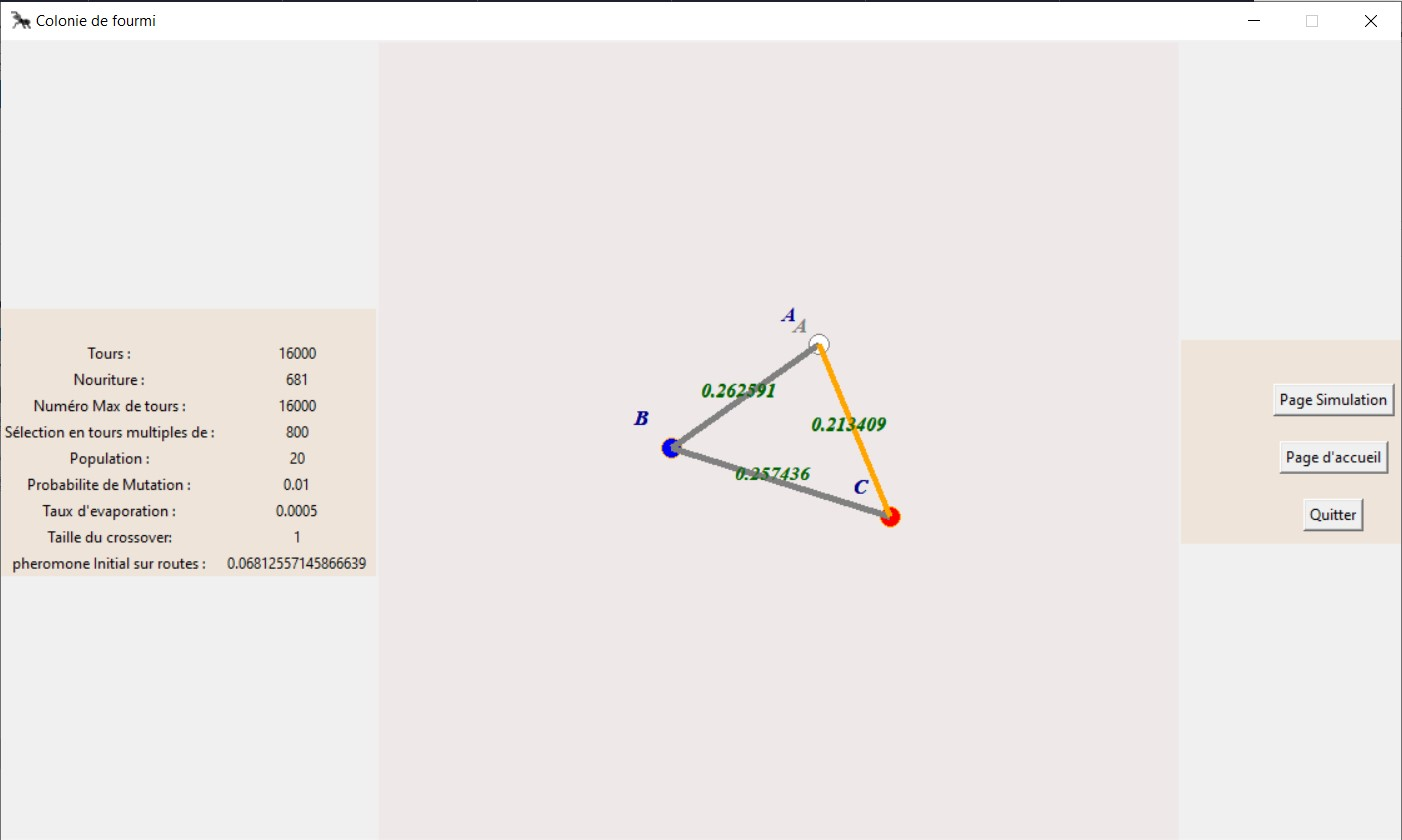
\includegraphics[width=0.8\linewidth]{triangle-mauvaise-solution.jpg}
    \caption{ exemple de graphe cyclique }
    \label{Dim}
\end{figure}\\

la figure ce-dessous montre le contraire, vu que nous avons choisi des bonnes paramètre , nous conclurons que le choix de paramètre à un impact sur la solution 

Les fournis qui sont perdu dans un boucle il ne représente pas des fournis de bonne explorateur.

\begin{figure}[H]
    \centering
    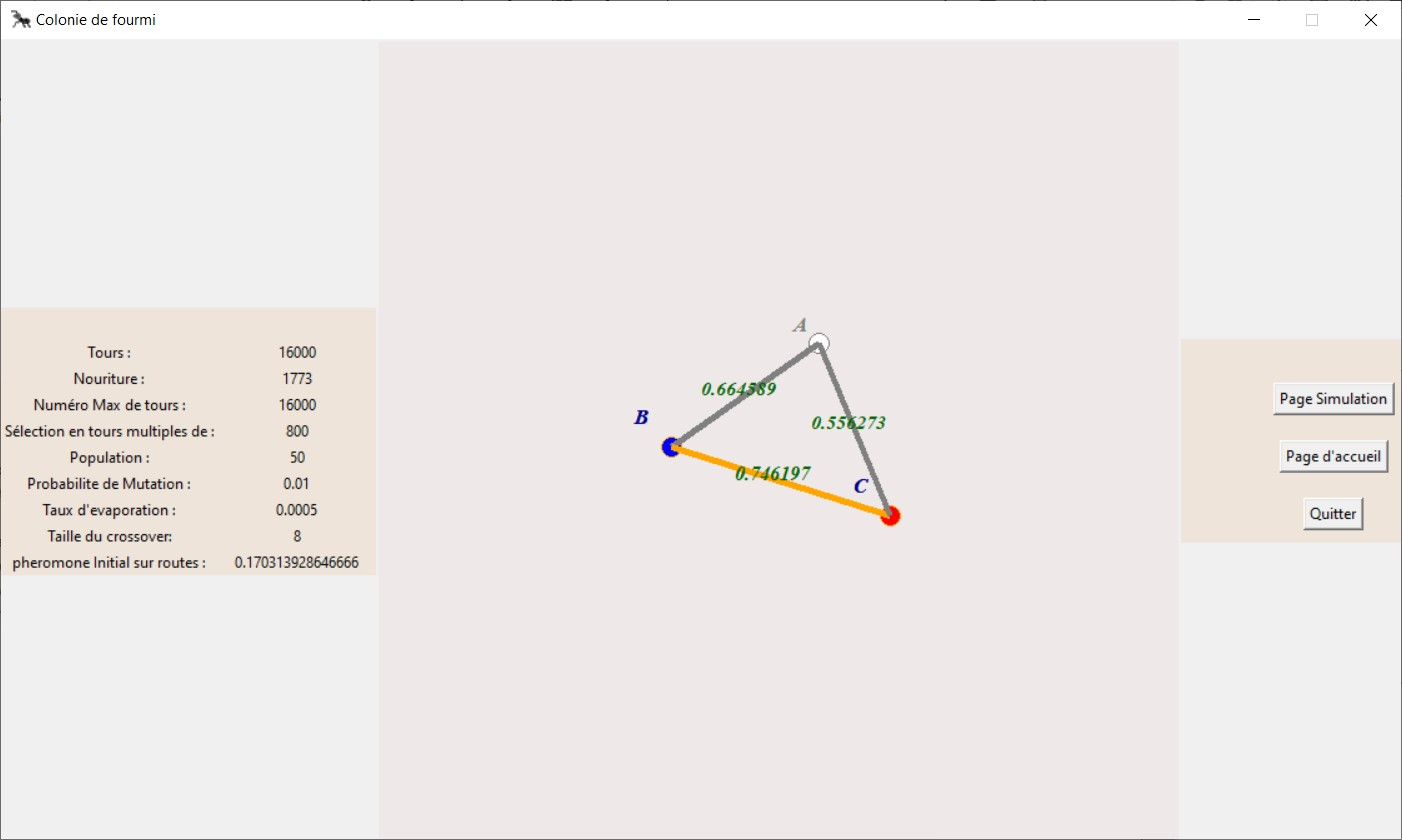
\includegraphics[width=0.8\linewidth]{ triangle-bonne-solution.jpg}
    \caption{ exemple de graphe cyclique }
    \label{Dim}
\end{figure}\\



En ce qui concerne le tri, le tri se fait deux fois par rapport les travailles et les explorateurs par conséquence la fonction croissement (Crossover) généré deux enfants un par représente les travailleurs et un ’autre représente les explorateurs.

\newpage
l'une des spécificité de les algorithme génétique c'est que il ne sont pas exacte mais il donnent une solution approximative, pour le probleme de colonie de founie il y a pour beaucoup de situation l'algorithme il ne trouve pas de solution pour il est nécessaire de faire plusieurs tentative pour trouver les bonnes parametre qui permet à l'algorithme de trouver une solution faisable.


\section{Implémentation}

L'implémentation du programme a été faite avec la langage Python 3.8.1. Le documentation a été fait en utilisant docstrings et des commentaires. On a aussi fait le design du code de tel façon  à aider la compréhension, en choisissant les nome des variables, attributs et méthodes qui explicitent notre solution. Le code est montré dans les sous-sections suivants:

La mise en ouvre pour la modélisation utilise la programmation orientée objet. On a utilisé quelques composants du module  Python “Tkinter”, permettant de créer des interfaces graphiques.. 

Pour bien modéliser notre problème nous avons utiliser UML

 \begin{figure}[H]
    \centering
    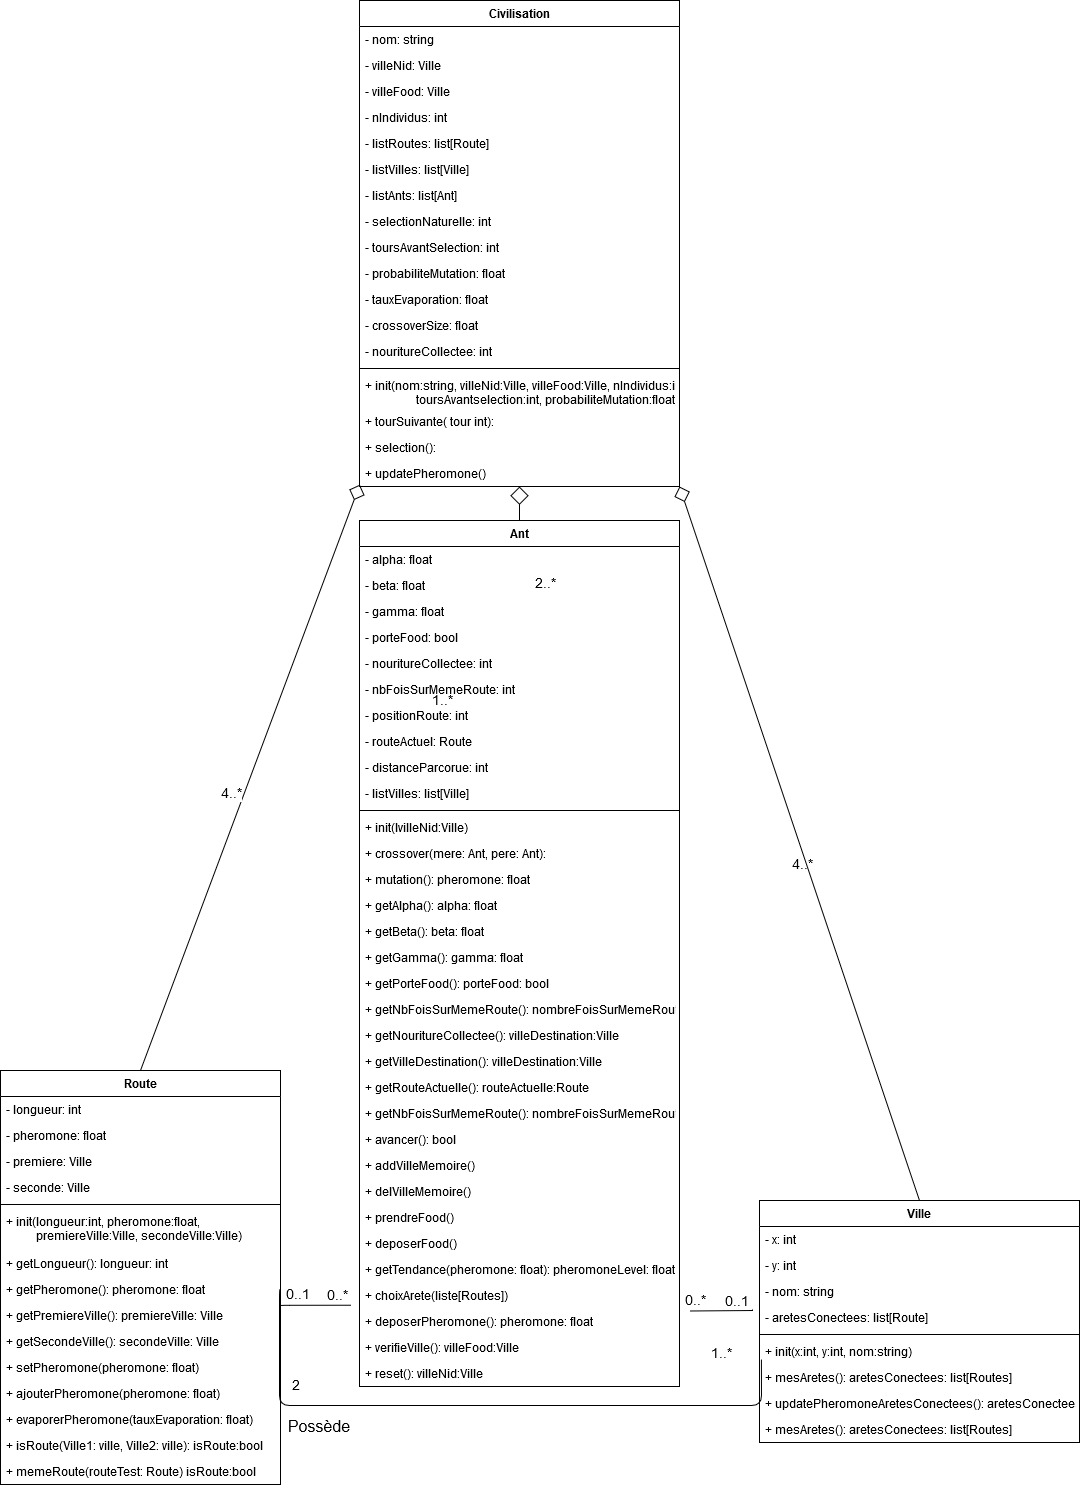
\includegraphics[width=0.8\linewidth]{UML-Civilisation-Fourmi-Route-Ville-UML.jpg}
    \caption{  Diagramme UML  }
    \label{Dim}
\end{figure}\\

\subsection{ville.py}

\inputminted{python}{scr/ville.py}

\subsection{route.py}

\inputminted{python}{scr/route.py}

\subsection{ant.py}

\inputminted{python}{scr/ant.py}

\subsection{civilisation.py}

\inputminted{python}{scr/civilisation.py}

\subsection{\text{zoneaffichage.py}}

\inputminted{python}{scr/zoneaffichage.py}

\subsection{\text{file\_manager.py}}

\inputminted{python}{scr/file_manager.py}

\subsection{\text{test\_colonie\_fourmi.py}}

\inputminted{python}{scr/test_colonie_fourmi.py}

% La fourmi arrive à la SOURCE en utilisant la ROUTE(SOURCE, AVANTSOURCE)
% On ajouté SOURCE sa mémoire;

% La ROUTE devient (villeActuel = self.__routeActuel.getSecondVille, derniere ville de la liste)

% (self.__premiereVille == ville1 and self.__secondeVille == ville2) or (self.__premiereVille == ville2 and self.__secondeVille == ville1)


% On a crée un diagramme UML (figure \ref{fig: Label du diagramme UML}) avec tous les classes qu'on a eu besoin pour arriver au cahier de charges. On crée une classe Jouer et une classe Historique pour stoker les informations du jouer et de ses parties (fichier jouer.py). Les classes StartPage, PageNon, PageHstorique et PageGame, qui héritent de la classe Frame, bien comme les classes MonBouton, Zoneaffichage et FenPrincipale font l'implementation de la interfaces graphiques et aussi de la gestion des parties (cf. pendu\_interface.py)

% %------ Pour insérer et citer une image centralisée -----

% %\insererfigure{img/TD5_UML.jpg}{13cm}{Diagramme UML}{Label du diagramme UML}
% % Le premier argument est le chemin pour la photo
% % Le deuxième est la hauteur de la photo
% % Le troisième la légende
% % Le quatrième le label

% %Ici, je cite l'image \ref{fig: Label du diagramme UML}



% \section{Implementation}

% L'implementation du programme a été faite avec la language Python 3.7. Le docummentation a été fait en utilisant docstrings et des commentaires. On a aussi fait le design du code de tel façon  à aider la compréhension, en choisissant les nome des variables, attributs et méthodes qui explicitent notre solution. Le code est montré dans le topique suivant:

% \subsection{jouer.py}

% \inputminted{python}{scr/jouer.py}

% \subsection{pendu\_interface.py}

% \inputminted{python}{scr/pendu_interface.py}


% \subsection{Analyse des résultats}

% \subsubsection{test\_jouer.py}

% Tout d'abord, un code de test seulement pour les classes "Jouer" et "Historique" a été élaboré. Un joueur a été simulé à travers de la création d'un objet "Jouer1" de la classe "Jouer" et des appels à ses méthodes.

% \inputminted{python}{scr/test_jouer.py}

% %------ Pour insérer et citer une image centralisée -----
% \insererfigure{img/Sortie_du_code_test_jouer_et_fichier.jpg}{12cm}{Sortie du code test\_jouer.py et fichier "Jouer1 ECL.txt" généré}{Label du Sortie du code Part 1}
% % Le premier argument est le chemin pour la photo
% % Le deuxième est la hauteur de la photo
% % Le troisième la légende
% % Le quatrième le label

% \subsubsection{Test de l'interface graphique}

% On lance les 2 codes pour démarrer une partie. Après avoir saisi notre nom (cf. figure \ref{fig: Label EcranNom}), voici l'interface sur laquelle on arrive (figure \ref{fig: Label Interface accueil}).

% \begin{figure}[H]
% \insererfigure{img/EcranNom.png}{4cm}{Interface Choisir nom}{Label EcranNom}
% \end{figure}

% \begin{figure}[H]
% \insererfigure{img/EcranAccueil.png}{9.6cm}{Interface d'accueil}{Label Interface accueil}
% \end{figure}

% En cliquant sur "nouvelle partie", on lance une partie et on arrive sur l'écran suivant :

% \begin{figure}[H]
% \insererfigure{img/NouvellePartie.png}{9.6cm}{Ecran de début de partie}{}
% \end{figure}

% A la fin du jeu, suivant si l'on a gagné ou perdu, on a les écrans suivants :

% \begin{figure}[H]
% \insererfigure{img/PartieGagne.png}{9.6cm}{Ecran en cas de victoire}{}
% \end{figure}

% \begin{figure}[H]
% \insererfigure{img/PartiePerdu.png}{9.6cm}{Ecran en cas de défaite}{}
% \end{figure}

% On peut ensuite revenir sur l'écran d'accueil et consulter notre historique, qui se présente sous la forme suivante : 

% \begin{figure}[H]
% \insererfigure{img/Historique.png}{9.6cm}{Historique}{}
% \end{figure}

% Cet historique est enregistré dans un document texte associé à chaque nom de joueur :

% \begin{figure}[H]
% \insererfigure{img/DossierHistorique.png}{9.6cm}{Document associé au joueur "Brice"}{}
% \end{figure}

% %------ Pour insérer et citer une image centralisée -----

% Remarque : Pour que le code fonctionne, il faut que les images disponible sur pédagogie, la liste des mots ainsi que les codes soient enregistré suivant le chemin suivant : 

% \begin{figure}[H]
% \insererfigure{img/Chemin.png}{9.6cm}{Chemin pour enregistrer les données}{}
% \end{figure}

% Les images montrent le fonctionnement du jeu. Il est bien fonctionnel d'après les différents tests
% réalisés présentés et satisfait au cahier des charges. Les classes StartPage, PageNon, PageHstorique et PageGame, qui héritent de la classe Frame, nous ont permit de avoir plusieurs pages pour le jeu, chacune d'elles contenant les informations pertinentes respectives pour le joueur, sans avoir besoin de créer plusieurs fenêtres. Cela crée une ambiance plus agréable pour l'utilisateur.

\end{document}
